\section{Dialect Generation}
\label{sec:dial}

Dialect generation is to derive variations from standard protocols. 
The generated dialects are only partially compatible to the original protocols. 
Communicating by using protocol dialects can reduce attack surface and amplify contrast for anomalies. 
In this section, we will first discuss challenges faced during dialect generation in Section~\ref{sec:dial_challenges}. 
We will then use a protocol implemented in OpenVPN and 
its three dialects to motivate our technique design in Section~\ref{sec:openvpn}. 
Finally, we will present our proposed techniques in Section~\ref{sec:dial_tech}. 



\subsection{Design Criteria}
\label{sec:dial_challenges}

Dialect generation takes a protocol implementation as input 
and mutates the core protocol state machine, 
protocol peripheral features and transferred messages 
to generate a new protocol implementation. 
An ideal dialect generation technique needs to satisfy the following three criteria. 

\textbf{Correctness.} 
Different from mutants in mutation testing~\citep{mtest,mtest2}, generated dialects are still functional programs. 
Faced with complicated control flow, data dependence and data structure in the input protocol implementation, 
it is very difficult for a dialect generation technique not to introduce bugs during protocol mutations. 


\textbf{Consistency.}
Protocols usually involve two or more than two parties exchanging messages between each other.
The implementations for these involved parties may or may not be in the same code base. 
During dialect generation, all corresponding parties need to be identified and modified coordinately. 


\textbf{Diversity.}
If a dialect space is too small, it is very easy to exhaust all possible dialects inside the space.
An ideal dialect generation technique must be able to create a large dialect space systematically. 


Our proposed technique tackles this challenging problem from three aspects. 
First, we design a suite of comprehensive static analysis to conservatively mutate a protocol
implementation without introducing bugs. 
Second, we apply memory layout analysis and value set analysis 
to match sent and received messages 
and further identify core state machines, which communicate with each other and may not be in the same code base. 
Third, we create a set of mutation primitives on core state machines, 
protocol peripheral features and transferred messages, 
whose combinations can create a fairly large dialect space. 


\subsection{Preliminary Exploration: Case Study and Key Observation}
\label{sec:openvpn}

In this part, we will use a protocol implemented in OpenVPN 
and three manually created dialects as motivating examples 
to demonstrate the potential of dialect generation. 
Particularly, we will answer the following questions using these examples:

(1) Which parts of protocol implementation need to be changed in order to generate a dialect?
(2) Is it too difficult to generate a protocol dialect automatically?
(3) If it is not too difficult, where are technical challenges?



\begin{figure*}[!htb]
\centering
\subfloat[The Orginal Protocol]{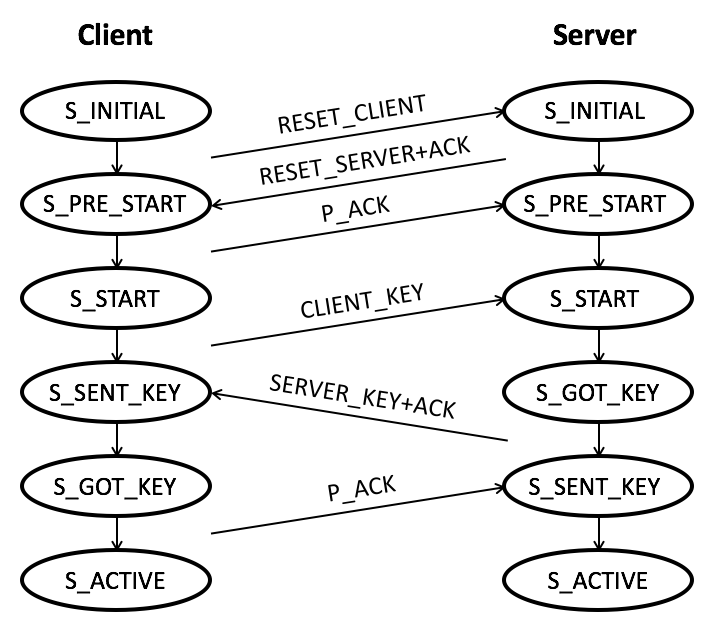
\includegraphics[width=0.24\linewidth]{figure/openvpn_protocol}\label{fig:openvpn_protocol}} 
\subfloat[Opcode Mutation]{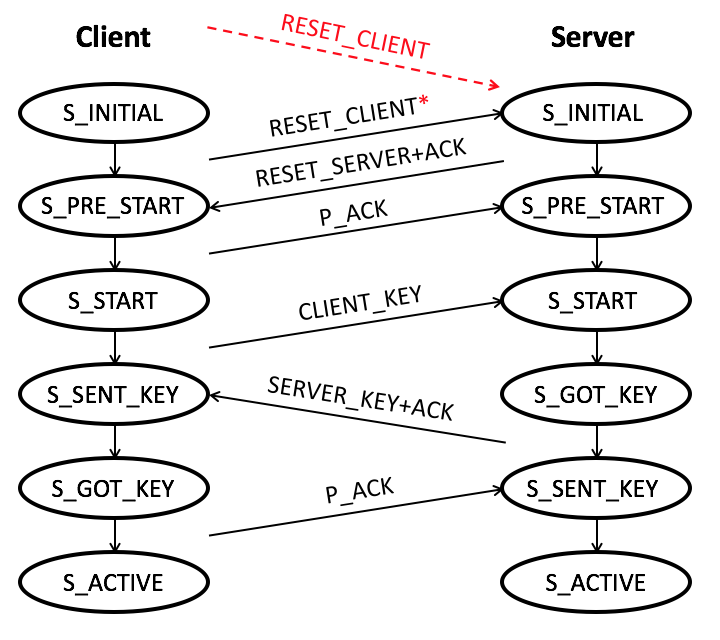
\includegraphics[width=0.24\linewidth]{figure/mutation1}\label{fig:mutation1}}
\subfloat[State Addition]{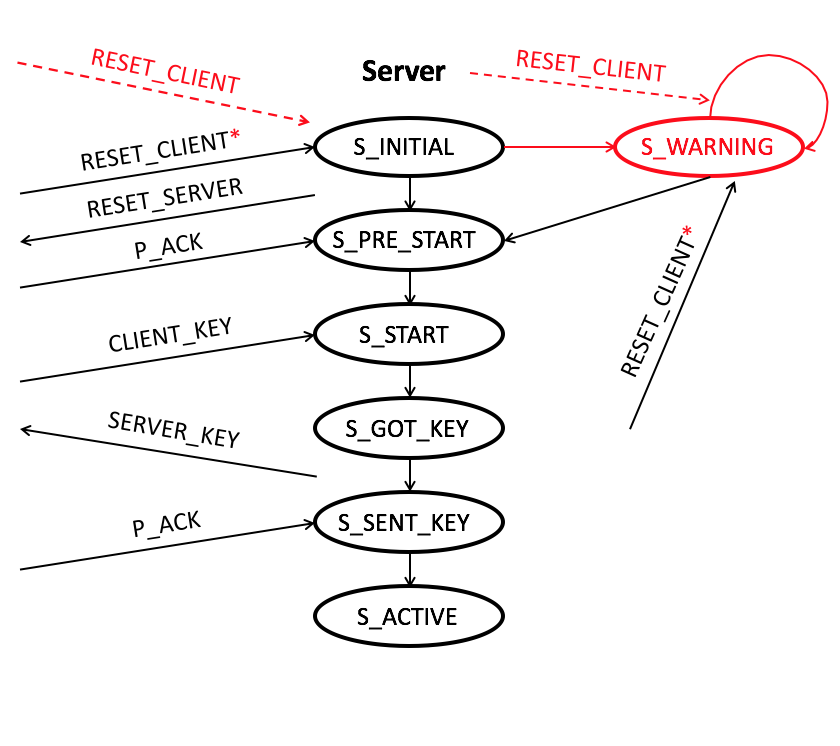
\includegraphics[width=0.24\linewidth]{figure/mutation2}\label{fig:mutation2}} 
\subfloat[Dialogue Addition]{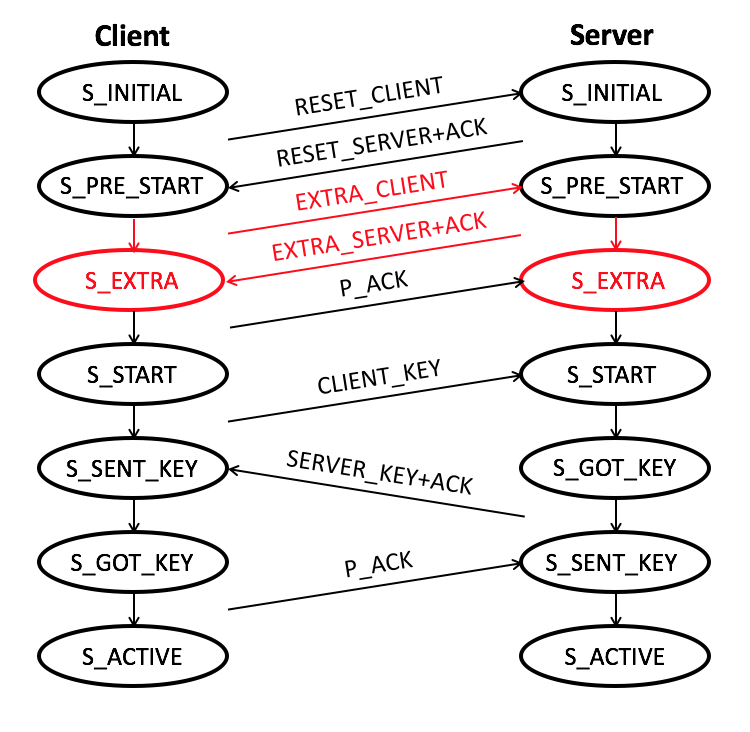
\includegraphics[width=0.24\linewidth]{figure/mutation3}\label{fig:mutation3}}\\ 
\vspace{-0.1in}
\caption{The OpenVPN protocol to establish a VPN tunnel and its dialects.
(\Code{RESET_CLIENT}, \Code{RESET_SERVER} and \Code{P_ACK} are defined opcodes in OpenVPN. 
 \Code{CLIENT_KEY} and \Code{SERVER_KEY} are exchanged 
  keys.
 \Code{P_ACK} is explicit acknowledgement. 
 \Code{ACK} represents implicit acknowledgement.
 Exchanged keys are encrypted and decrypted by OpenSSL libraries.
 Encrypted keys are larger than a UDP or TCP packet, 
 so they are splitted into multiple packets in the real implementation.
 For simplicity purpose, we only use one packet to represent one encrypted key. 
 For each dialect, mutated parts are colored in red.)} 
\label{fig:openvpn} 
\end{figure*} 

{\textbf{Background and the Original Protocol (Figure~\ref{fig:openvpn_protocol})}}
OpenVPN~\citep{openvpn-wiki,openvpn} is an open-source implementation for virtual private network. 
OpenVPN can be configured to either use TCP or UDP. 
It implements its own reliability layer to acknowledge and sequentialize received packets.  
Control and data packets are exchanged between OpenVPN client and OpenVPN server 
to establish a VPN tunnel and transfer data through the tunnel respectively. 
We will use the protocol to establish a VPN tunnel 
to demonstrate the basic ideas behind dialect generation. 

The process to establish a tunnel is shown in Figure~\ref{fig:openvpn_protocol}.
The first stage of the process is a three-way handshake, 
and then keys are exchanged in the second stage. 
Both of these two stages start with a packet from client and end with an ACK packet from client. 
A received package can be explicitly acknowledged by an ACK packet,
or implicitly acknowledged by inserting the packet id 
of the received packet into a packet to be sent to the other side.
All packets are acknowledged in each stage.  
State transitions are almost the same for both client and server, 
except that client will enter \Code{S_SENT_KEY} state firstly and then \Code{S_GOT_KEY}, 
while server does just the opposite. 


In terms of implementation, 
both client and server maintain its own finite-state machine (FSM).
The state variable is an integer field of a structure for both client and server.
Without changing the type of the state variable, 
there are in total $2^{32}$ possible state variable values. 
State variable values from $-1$ to $7$ are already used by the current OpenVPN implementation. 
Opcode, occupying $5$ bits in each exchanged packet, controls state transitions. 
In total, there are $2^5$ possible opcode values and $9$ of them are already used. 
As we mentioned earlier, OpenVPN implements its own reliability layer. 
FSMs on both client and server read received packets 
from the reliability layer to conduct state transitions, 
and write packets into the reliability layer to send packets to the other side. 


{\textbf{Opcode Mutation (Figure~\ref{fig:mutation1})}}
%For the first dialect, 
We change the opcode of the initial packet to \Code{RESET_CLIENT*}.
Since opcode values from 1 to 9 have already been used by the current implementation,
we set \Code{RESET_CLIENT*} to be 10.
There are 4 places in the implementation where the original opcode value is used explicitly, 
including 3 if-conditions to check whether an incoming packet is the initial packet from client on the server side 
and one assignment to set opcode value for the initial packet on the client side. 
We change these 4 places to use \Code{RESET_CLIENT*}.
There is another place to conduct sanity check for opcodes of all incoming packets. 
Packets without valid opcodes will be discarded 
and will not be processed by the FSMs on both client and server.
We change this part to accept packets with opcode \Code{RESET_CLIENT*} 
and filter out packets with opcode \Code{RESET_CLIENT}.
After applying the first dialect, 
server will not reply any packet to client trying to 
establish a VPN tunnel by using the original protocol. 



{\textbf{State Addition (Figure~\ref{fig:mutation2})}}
%For this dialect, 
We consider both \Code{RESET_CLIENT} 
and \Code{RESET_CLIENT*} as valid opcodes. 
We add an extra state, \Code{S_WARNING}, to the server FSM. 
When server receives a packet with opcode \Code{RESET_CLIENT}, 
the server FSM will change its state to \Code{S_WARNING}. 
A warning message or log could be generated for system administrators during this state transition.
When server receives a packet with opcode value \Code{RESET_CLIENT*},
the server FSM will transit to \Code{S_PRE_START} and start to establish a VPN tunnel.
In the loop implementing the server FSM, we add an if statement with condition to be true 
when the state is either \Code{S_INITIAL} or \Code{S_WARNING} 
and the opcode of the incoming packet is \Code{RESET_CLIENT}. 
Inside the true branch, we set the state variable to be \Code{S_WARNING} 
and update the reliability layer to remove the incoming packet 
from a list containing packets to be acknowledged later. 
The last place we change is to modify the condition controlling the transition from \Code{S_INITIAL} 
to \Code{S_PRE_INITIAL} to enable transition from \Code{S_WARNING} to \Code{S_PRE_INITIAL}.



{\textbf{Dialogue Addition (Figure~\ref{fig:mutation3})}}
%For the third dialect, 
We change the three-way handshake into a five-way handshake
by adding an extra state for both client and server FSMs and two exchanged messages. 
We change the opcode sanity check to accept packets with opcode \Code{EXTRA_CLIENT} 
and \Code{EXTRA_SERVER}. 
We double the time limit required to finish the handshake. 
Inside the loop implementing the server FSM, we add an if statement for the transition from 
\Code{S_PRE_START} to \Code{S_EXTRA}. 
We add codes to write a packet with opcode \Code{EXTRA_SERVER} 
into the reliability layer when the transition happens. 
The packet will be sent out later by other parts of the program. 
We also change the condition originally controlling the transition from \Code{S_PRE_START} to \Code{S_START}. 
When the new condition is satisfied, 
state will transit from \Code{S_EXTRA} to \Code{S_START}. 
Similar changes are also made for the client side. 


The OpenVPN protocol and the three dialects can help us answer the questions asked earlier.

(1) To generate a dialect, we may need to change values sets of packet opcodes and state variables. 
If this happens, we also need to change related sanity check. 
Inside the loop implementing a FSM, we may need to synthesize codes 
to conduct new state transitions,
and we may also need to synthesize codes to send packets with new opcodes. 

(2) Possible opcode values and state variable values 
are usually constant integers or enumerated values.  
It is not difficult to identify value sets for opcodes and state variables through static analysis. 
It is not difficult to mutate the value sets and related sanity check either. 
When an implemented FSM reads or sends a packet, 
it usually relies on high-level function calls. 
In our OpenVPN example, the client and server FSMs read packets from the reliability layer 
and send packets by writing into the reliability layer. 
If we can identify network I/O functions, 
it is not difficult to synthesize codes to read and send packets.
To sum up, it is feasible to design a tool to automatically generate protocol dialects. 


(3) We have already observed technical challenges through manually creating the three dialects. 
First, references to opcodes and state variables may scattered all over a protocol implementation. 
Take the current OpenVPN implementation as an example, 
the opcode sanity check is 700 lines away from the function implementing the FSM. 
We need to identify all of the references and make necessary changes. 
Second, different implementations may have their own high-level network I/O functions.
For example, OpenVPN has its own reliability layer between protocol FSMs 
and low-level network system calls. 
We need to identify proper customized network functions 
in order to synthesize codes to send and receive packets. 


\subsection{Proposed Techniques}
\label{sec:dial_tech}

Following the initial exploration above,
we divide our dialect generation into three stages:
(1) protocol mutation design and validation;
(2) program analysis and synthesis design and implementation; 
and (3) systematically mutation testing for new dialects. 


\subsubsection{Research Task 1: Protocol Mutation Design and Validation}


\begin{table}[h!]
  \centering
  \small
  \begin{tabular}{lccc}
    \toprule     
   {\textbf{Elements}}           &  \multicolumn{3}{c}{\textbf{Mutations}}\\              
    \cmidrule(lr){2-4}
                                 &  Addison     &   Removing    &    Revision    \\
    \midrule 
    State                        & \ding{55}    & \ding{55}     &  \ding{51}     \\
    Transition                   & \ding{51}    & \ding{51}     &  \ding{51}     \\
    Message                      & \ding{51}    & \ding{51}     &  \ding{51}     \\
    \bottomrule
   \end{tabular}
  \caption{Protocol Mutation Operators. (\ding{51}: can be used as a first-order mutation; \ding{55}: cannot be used as a first-order mutation.)}
  \label{tab:operators}
\end{table}

{\textbf{Protocol Mutation}}
There are three basic types of elements for a given protocol: 
state, transition and message. 
For each type, we can add an extra element, remove an element and revise an existing element.
Therefore,
we define 9 types of protocol mutation operators for all possible combinations 
between a type of protocol elements and a type of changes. 
Following previous works in mutation testing area~\citep{higher-order},
we consider only applying one mutation operator once as first order mutation, 
and applying mutation operator multiple times as higher order mutations. 
As shown in Table~\ref{tab:operators}, 
state addison and removing cannot be used as first order mutation,
since we also need to add or remove transition starting and ending at the state. 
Opcodes inside messages control state transition, 
so message revisions are about changing opcodes, as shown in Figure~\ref{fig:mutation1}.  
A state transition could happen unconditionally or not depend on an incoming message, 
so transition addison could be used as first order mutation. 


{\textbf{Mutation Validation}}
We also define several graph theory based rules to check whether
a protocol mutation contains logical errors 
before conducting code transformations. 
Several examples for our checking rules are listed as follows.
Each state must be reachable from the initial state, 
and the final state must also be reachable from every other state.
For each involved FSM, every transition is deterministic, such as
two transitions from the same state cannot have the same condition. 
There are no circular wait messages among communicating parties to avoid deadlock. 


